In order to implement the application, first of all, a new project has to be created in Eclipse. This project is going to be a Papyrus project (figure \ref{fig:Papyrus Project}).

\begin{figure}
\centering
{\includegraphics[scale=0.3]{./chapter4/projPapyrus/Selection_001.png}}
\caption{New Papyrus Project}
\label{fig:Papyrus Project}
\end{figure}

The first field that has to be specified is the Architecture Context. Here, the default values are the right ones as an UML model is what is required to implement with Papyrus (figure \ref{fig:Architecture Context}).

\begin{figure}
\centering
{\includegraphics[scale=0.3]{./chapter4/projPapyrus/Selection_002.png}}
\caption{Architecture Context}
\label{fig:Architecture Context}
\end{figure}

After that, the name of the project has to be defined. Due to the fact that it is going to implement an application called Great Seller, the name of the Papyrus project is going to be greatSellerApp (figure \ref{fig:Project Name Definition}).

\begin{figure}
\centering
{\includegraphics[scale=0.3]{./chapter4/projPapyrus/Selection_003.png}}
\caption{Project Name Definition}
\label{fig:Project Name Definition}
\end{figure}

The next step is to select the representation kind and to choose the StreamGen profile. StreamGen requires Papyrus to make a class diagram representation and, as the StreamGen project is already in the Eclipse workspace, the profile can be found browsing in the workspace (streamgen/profile/StreamUML.profile.uml). As it can be seen in the figure \ref{fig:Representation Kind}.

\begin{figure}
\centering
{\includegraphics[scale=0.3]{./chapter4/projPapyrus/Selection_004.png}}
\caption{Representation Kind}
\label{fig:Representation Kind}
\end{figure}

Finally, we can finish with the new Papyrus project initialization (figure \ref{fig:Papyrus Project Definition}).

\begin{figure}
\centering
{\includegraphics[scale=0.3]{./chapter4/projPapyrus/Selection_005.png}}
\caption{Papyrus Project Definition}
\label{fig:Papyrus Project Definition}
\end{figure}

The next step is to define the model in the class diagram in order to specify that the application is going to be a Flink application. Then, first of all, we have to create a model node in the greatSellerApp.di file. This node is going to be called greatSeller as it is the object representing the whole application. Once the node is inserted, the properties of such node must be specified. More in detail, the Flink application stereotype has to be applied. In this case, the properties of the model has to be the default ones then nothing else must be done with the model node.

The next step is to add the data types that the application is going to need. In order to do this, a package node has to be inserted inside the Flink application model node. This package is called greatSellerDataTypes and a stereotype has to be applied as in the previous case. First of all, inside the properties window, in the profile field, the applied stereotype is defined. Inside this package all the datatypes that the application requires have to be inserted. The first data type is the InputTransactions which is composed of a transaction id (integer), a data subject (string), an amount (double) and a recipient id (string). The second data type is the IssuedTransactions which contains the data subject (string) and the number of transactions performed by such data subject which can be seen by means of the variable NTransactions (integer). The third data type is the SpentAmount which is composed of the data subject (string) and the total amount of money spent by the data subject which can be seen by means of the variable TotalAmount (double). Finally, the last data type is the NumberUsers which contains the number of users who spent more than 1000 dollars and it is represented by means of the variable NTopUsers (integer). Then, we need to insert one DataType node inside the package created in the previous step with each of these data types. Each data type can be seen as a tuple which is composed by several values. The name of the DataType node is going to be the same that the one corresponding to the tuple and each of the values that compose the tuple are going to be a property inside of the owned attributes that are specified in the UML field of the properties of each DataType node.

\begin{table}[h!]
\centering
	\begin{tabular}{||c|c|c||} 
	\hline\hline
	DataType & Properties & PropertyType \\ [1ex] 
	\hline\hline
	InputTransactions & transactionId & integer  \\
	& dataSubject & string  \\
	& amount & double  \\
	& recipientId & string  \\
	\hline
	IssuedTransactions & dataSubject & string  \\
	& nTransactions & integer \\
	\hline
	SpentAmount & dataSubject & string  \\
	& totalAmount & double \\
	\hline
	NumberUsers & NTopUsers & double  \\
	\hline\hline
	\end{tabular}
\caption{DataTypes Composition}
\label{DataTypes Composition}
\end{table}

\section{Files Generation}

\subsection{Source Files Generation}
In order to generate the text file that feeds the Great Seller DIA, two Python codes have been developed. In addition, a Map Transformation is implemented in the DIA in order to split the input strings generated by the Python codes and to generate the InputTransaction data type.

The first Python code builds a Python list which represents the Great Seller stock of 25 products and it assigns to each product a price. Each product is represented with a dictionary variable that contains a name variable and a price variable. The name variable is a string with the word 'product' immediately followed by an integer number from 1 to 25 which points to the product of the stock. The price is an integer number between \$1 and \$200 which is assigned randomly. Once the name and the price are assigned to the dictionary, the product is added to the stock list. Finally, the Great Seller stock list is saved in a binary shelf file in order to be accessible from the other Python code.

The second Python code generates the strings that represent the tuples produced by each consumer. In order to generate such tuples an integer number for the transactionId is assigned following an increasing numerical order from 1 to the maximum number of generated transactions which is input by command line to the code, it can be 10, 100 or 1000. After that, randomly, one of the four possible data subjects (Bob, Carlos, Elisabetta and Michele) and a product from the stock saved in the binary shelf file are assigned. Finally, each value is added to a string where each of these values are separated by a comma. The generated string represents the tuple produced by each consumer and it is written in the text file which is called from the Great Seller DIA in order to feed it.

Once, the DIA inputs each of this strings in a non-parallel stream, a Map Transformation, taking advantage of the split Java method, splits the strings by the comma generating the InputTransaction data type which is composed of four fields: transactionId, dataSubject, amount and product.


\subsection{Java Codes Generation}

In order to generate the Java codes from the Papyrus model, first of all we need to create a new Java project in Eclipse (File -$>$ New -$>$ Java Project). This project is going to be called 'greatSellerCodes' as it can be seen in the figure \ref{fig:Java Project Creation}.

\begin{figure}
\centering
{\includegraphics[scale=0.3]{./chapter4/javaCodesGeneration/Selection_001.png}}
\caption{Java Project Creation}
\label{fig:Java Project Creation}
\end{figure}

Once the Java project is created, its structure has to be modified in order to allow to be compatible with Maven. As the figure \ref{fig:Java Project Initial Structure} shows, firstly the Java project is composed of a JRE System Library and a src folder. This src folder has to be deleted, leaving the Java project only with the JRE System Library as it can be seen in the figure \ref{fig:Java Project Final Structure}.

\begin{figure}
\centering
{\includegraphics[scale=0.3]{./chapter4/javaCodesGeneration/Selection_002.png}}
\caption{Java Project Initial Structure}
\label{fig:Java Project Initial Structure}
\end{figure}

\begin{figure}
\centering
{\includegraphics[scale=0.3]{./chapter4/javaCodesGeneration/Selection_003.png}}
\caption{Java Project Final Structure}
\label{fig:Java Project Final Structure}
\end{figure}

The next step is to create a source folder with a predefined structure as it is going to be specified now. Firstly, in the properties for the project, in the Java Build Path field, a folder has to added as the figure \ref{fig:Maven Project Structure Creation} specifies. In the default output folder a specific structure has to be written, greatSellerCodes/src/main/java. After this is written, the changes have to be applied and then click on 'Add Folder...'.

\begin{figure}
\centering
{\includegraphics[scale=0.3]{./chapter4/javaCodesGeneration/Selection_004.png}}
\caption{Maven Project Structure Creation}
\label{fig:Maven Project Structure Creation}
\end{figure}

In order to create the source folder, the java folder has to be selected and then click on 'OK' as it is shown in figure \ref{fig:Maven Project Source Folder Creation}. Then the changes have to be applied and, then, the window Properties for greatSellerCodes has to be closed (figure \ref{fig:Maven Project Properties}).

\begin{figure}
\centering
{\includegraphics[scale=0.3]{./chapter4/javaCodesGeneration/Selection_005.png}}
\caption{Maven Project Source Folder Creation}
\label{fig:Maven Project Source Folder Creation}
\end{figure}

\begin{figure}
\centering
{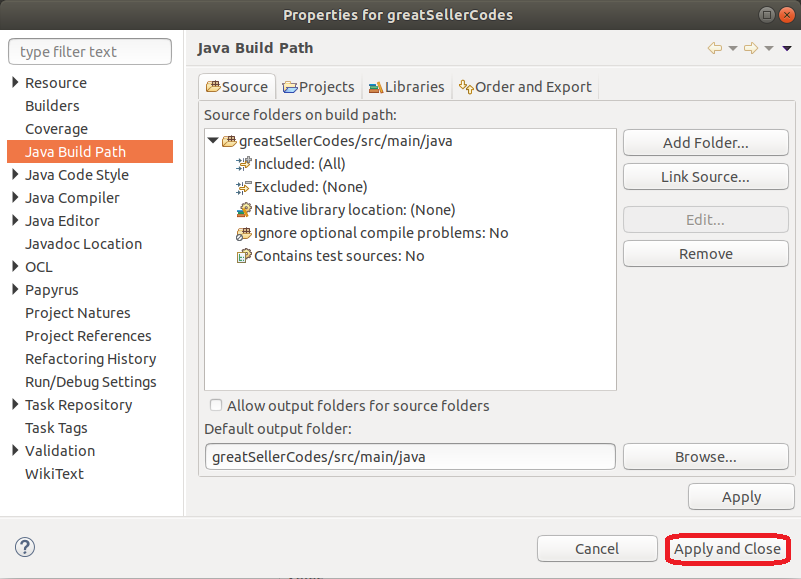
\includegraphics[scale=0.3]{./chapter4/javaCodesGeneration/Selection_006.png}}
\caption{Maven Project Properties}
\label{fig:Maven Project Properties}
\end{figure}

After these steps, the project folder should look like it is shown in the figure \ref{fig:Maven Project Structure} at the Package Explorer. And then, the project is ready to convert it into a Maven project. In order to do this, going to the 'Configure' option of the project and then clicking on 'Convert to Maven Project'. Then, a POM file has to be created and it is going to be created the default one as it can be seen in the figure \ref{fig:POM File Creation}. At this point, the structure of the project has to be the same that the one shown in the figure \ref{fig:Final Maven Project}.

\begin{figure}
\centering
{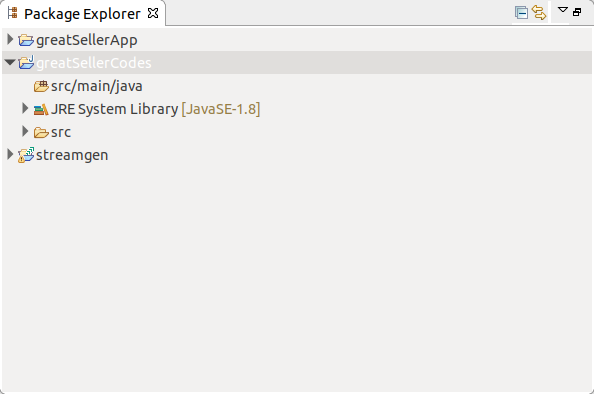
\includegraphics[scale=0.3]{./chapter4/javaCodesGeneration/Selection_007.png}}
\caption{Maven Project Structure}
\label{fig:Maven Project Structure}
\end{figure}

\begin{figure}
\centering
{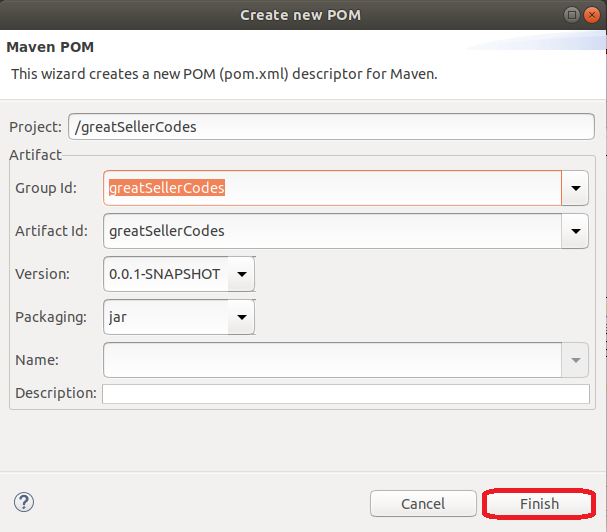
\includegraphics[scale=0.3]{./chapter4/javaCodesGeneration/Selection_008.png}}
\caption{POM File Creation}
\label{fig:POM File Creation}
\end{figure}

\begin{figure}
\centering
{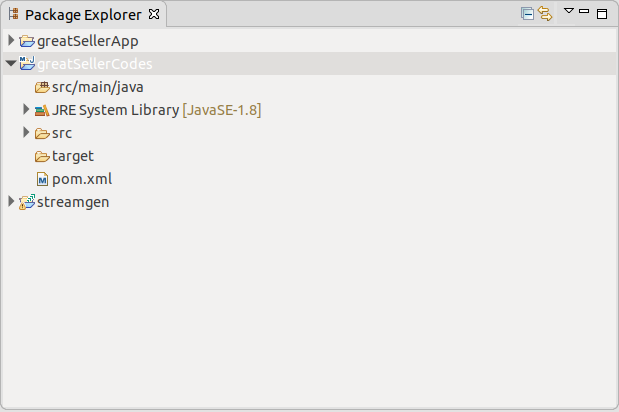
\includegraphics[scale=0.3]{./chapter4/javaCodesGeneration/Selection_009.png}}
\caption{Final Maven Project}
\label{fig:Final Maven Project}
\end{figure}

Now it is time to run the configuration (Run -$>$ Run Configurations...). In the figure \ref{fig:Run Configuration} is shown how this window has to be filled.

\begin{figure}
\centering
{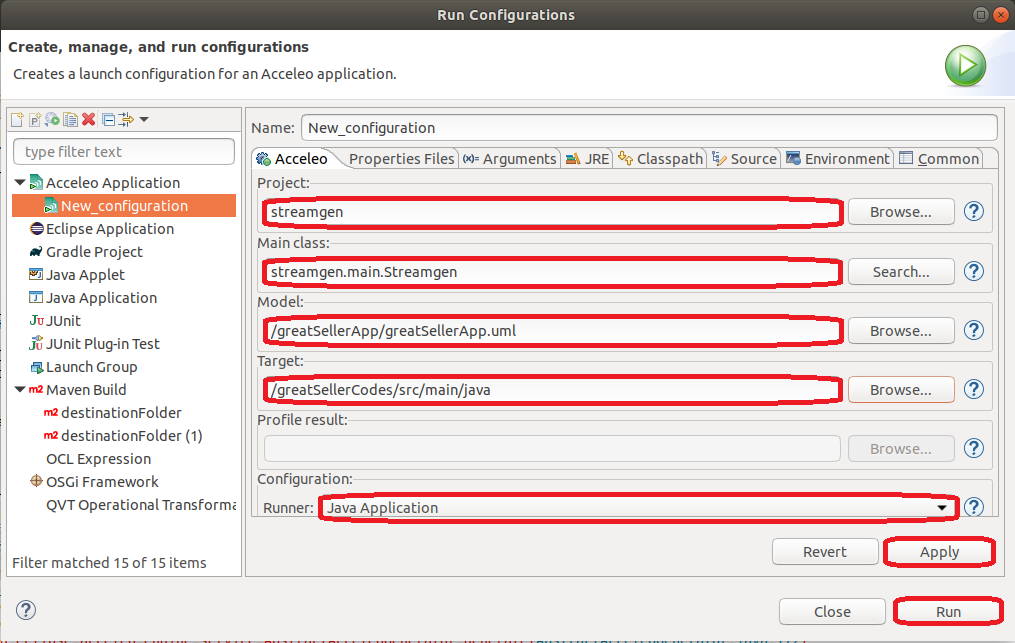
\includegraphics[scale=0.3]{./chapter4/javaCodesGeneration/Selection_010.png}}
\caption{Run Configuration}
\label{fig:Run Configuration}
\end{figure}

\section{Requirements}
The first requirements that are needed in order to develop the big data application is to install the corresponding versions of Eclipse, Papyrus and Acceleo. In spite of the application is able to work with other versions, some problems could appear because of the changes that they present. The models implemented in this document have been developed with the following versions:

\begin{itemize}
\item Eclipse 2019-03 (4.11.0).
\item Papyrus SysML 1.4 Feature	1.3.0.
\item Acceleo 3.7.8.201902261618.
\item m2e-Maven Integration for Eclipse (includes Incubating components) 1.11.0.20190220-2119.
\item Apache Flink 1.4.0.
\end{itemize}

\section{Privacy Policy Language}

StreamGen uses its own language in order to develop DIA. In this document, StreamGen language has been expanded in order to allow users to protect the streams with privacy policies. This expansion consists of a new data stream stereotype in order to specify which streams are protected and with which privacy policy type. Moreover, the sources that generate the Static Context Variables (SCV) and the rules written by the users are also added to the StreamGen language. SCV are going to be possibly supplied by different sources whilst privacy policies will be supplied only by one data source type. This sources are going to be inserted in a package which represents the external sources of the DIA.

\subsection{PrivacyProtectingStream}

StreamGen represents the flows of data flowing in DIA by means of UML metaclass Information Flow. This flows are known as streams and StreamGen allow to generate some different types as Keyed Stream or Windowed Stream. Each of these types have different characteristics and allow the users to generate different behaviors. Moreover, these different streams can be applied all together generating a stream which can be, as in this case, windowed and keyed.

Following this approach, a new stereotype has been added to the UML profile. This stereotype has been called PrivacyProtectingStream and it is a generalization of the DataStream stereotype, which in turn is an extension of the InformationFlow metaclass. This new stereotype is going to have some properties in addition to the property of the DataStream stereotype, isObservable. These properties are:

\begin{itemize}
\item ProtectedByVCP.
\item ProtectedByDSEP.
\item ProtectedStreamConf.
\end{itemize}

ProtectedByVCP and protectedByDSEP properties are added in order to specify how the DataStream is protected; if it is protected with a DSEP, with a VCP or if it is protected with both privacy policies.This is why these two properties are going to be boolean values. Moreover, the configuration of the generated protected stream, which is imported from the library, has to be specified. In order to define such configuration, a new DataType has been added to the UML profile. This DataType is called ProtectedStreamConfiguration and it is composed of seven properties: monitoringActive (Boolean), timestampServerIp(String), timeStampServerPort (Integer), topologyParallelism (Integer), simulateRealisticScenario (Boolean), allowedLateness (Integer) and logDir (String).

In the figure \ref{fig:PrivacyProtectingStream UML Profile}, the UML profile for the PrivacyProtectingStream is shown.

\begin{figure}
\centering
{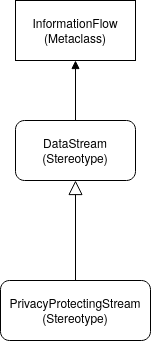
\includegraphics[scale=0.3]{./chapter4/umlProfile/PrivacyProtectingStreamUMLProfile.png}}
\caption{PrivacyProtectingStream UML Profile}
\label{fig:PrivacyProtectingStream UML Profile}
\end{figure}

\subsection{PrivacyPolicySources} % What about call this 'ExternalSources', this name is weird taking into account the PrivacyPolicySource

StreamGen uses a package called StreamDatatypes in order to collect all the DataTypes that are flowing through the streams. The DataTypes that are specified inside the package allow the users to specify the different values that are conveyed in a stream but inside the same tuple. Following these approach, a new package called PrivacyPolicySources has been added to the UML profile in order to collect all the sources involved in the privacy policies applications, SCV sources and user privacy policies.

These sources are not going to be connected directly to the streams or to the transformations of the DIA but they are going to allow the users to specify from where the different variables required to protected the streams are taken. As they are not going to be connected, a package to put all of them together is added to the language.

In the figure \ref{fig:PrivacyPolicySources Package UML Profile} can be seen the UML profile of this package.

\begin{figure}
\centering
{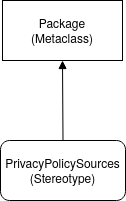
\includegraphics[scale=0.3]{./chapter4/umlProfile/PrivacyPolicySourcesUMLProfile.png}}
\caption{PrivacyPolicySources Package UML Profile}
\label{fig:PrivacyPolicySources Package UML Profile}
\end{figure}


\subsubsection{PrivacyContextSource}

Static Context Variables are required in order to know when an user specified privacy policy can be apply. These SCVs can be just an agent or many of them. This is why a wide variety of possibilities have been developeded in order to allow the users to choose the most appropriate SCV source. Such possibilities are:

\begin{itemize}
\item PrivContTextFileSource.
\item PrivContSocketSource.
\item PrivContKafkaSource.
\item PrivContFixedSource.
\end{itemize}

Following the approach of StreamGen with DataSource, a stereotype called PrivacyContextSource has been created as a generalization of the already existing DataSource stereotype. This new stereotype have four generalizations, the four possibilities to choose by the user when the SCV source has to be defined. Each of these four sources have its own properties. These properties have been defined taking into account the already existing data sources:

\begin{itemize}
\item TextFileSource.
\item SocketSource.
\item KafkaSource.
\end{itemize}

TextFileSource stereotype reads a file which contains all the input values of the DIA. When the user selects the stereotype,the path (pathToFile) from where the DIA must read the file has to be specified. PrivContTextFileSource works exactly in the same way, this stereotype contains a property called pathToFile (String) where the user will have to specify the path where the file with all the SCV tuples is located. SocketSource stereotype is connected to a port and to a host by means of the properties host (String) and port (Integer) that the user specifies when the stereotype is defined. Following this approach, PrivContSocketSource is connected by a port (Integer) and a host (String) to a server which supplies the SCV tuples.Finally, the KafkaSource is connected by means of kafkaBrokerIp (String) and kafkaBrokerPort (Integer) to a Kafka server. PrivContKafkaSource connects a DIA to a Kafka server that provides the SCV tuples by means of two properties as in the case of the KafkaSource.

In case of PrivContTextFileSource and PrivContSocketSource, when the code is generated a NonParallelStream called contextString which contains the SCV tuples (Strings) is introduced into the DIA. This stream is automatically sent to a map transformation which is imported from the library. This map transformation parses contextString to a stream composed with the DataType specified by the user. This DataType should contain the same data that each of the strings but the values are split by the comma in order to have each of the values independently. Moreover, this stream is called contextStream and it will be used to apply the privacy policies.

Finally, PrivContFixedSource is a source imported from the library which allows the users to specify only one SCV source. In order to do this, when the user is defining the UML model of the DIA, three properties must be specified. This three properties are fixedUser (String), fixedRole (String) and fixesPuporse (String) which allow to specify the static or fixed SCV source.

In case of PrivContKafkaSource and PrivContFixedSource the contextStream with the user specified DataType is directly generated without applying any transformation.

\subsubsection{PrivacyPolicySource}

In addition to SCVs, StreamGen requires some user specified rules to guarantee privacy. These rules are going to be written in a YAML file that must be imported to the DIA in order to feed the privacy library. In order to do this, the library snakeyaml (org.yaml.snakeyaml.Yaml) is used. This is the unique type of sources for such purpose as the rules are supposed to be stored in a YAML file.

Following the approach of DataSource stereotype, a new stereotype called PrivacyPolicySource is created as a generalization of the DataSource stereotype. The goal with this stereotype is to have the possibility to add different type of sources as currently is happening with the SCV source. From the PrivacyPolicySource stereotype, a new generalization is created in order to make the relationship with a new stereotype called PrivPolYamlFileSource. This stereotype represents the insertion of the YAML file to the DIA. In order to specify the path where the YAML file is located, a new property (pathToFile, String) is added to the stereotype. With this property, the user is able to define the location where the file is stored and from where the DIA must read the privacy policy rules written by the user.

In the figure \ref{fig:PrivacyPolicySources Classes UML Profile} can be seen the language of the PrivacyContextSource and PrivacyPolicySource represented in a UML profile diagram.

\begin{figure}
\centering
{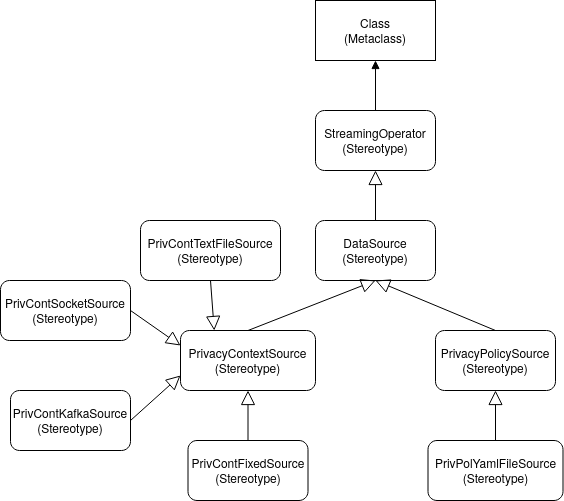
\includegraphics[scale=0.3]{./chapter4/umlProfile/PrivacyPolicyDataSourceUMLProfile.png}}
\caption{PrivacyPolicySources Classes UML Profile}
\label{fig:PrivacyPolicySources Classes UML Profile}
\end{figure}

\section{Privacy Policy Translation}

The UML metamodel that specifies the language for the privacy policies must be by the user in order to create the UML class diagram of the DIA. This diagram is used by Acceleo in order to generate the final code which runs in Flink. In this section this step is explained. Furthermore, all along this section an assumption is taken. This assumption is that the UML file generated by Papyrus is going to contain all the packaged classes in the following order:

\begin{enumerate}
\item Sources.
\item Transformations.
\item Sinks.
\end{enumerate}

First of all, all the sources introducing data are going to be packaged as elements in the UML file that is generated by Papyrus. After them, all the transformations are packaged. Finally, all the sinks where the data must be stored are packaged. This assumption is similar to say that the DIA is built in order without adding transformations, sinks or sources after generating the DIA. This is important in order to generate a target code in order and without modifications of pieces of code once it has already been generated.

In addition to this assumption, the target code generated by means of StreamGen must be able to follow a structure that will generate the same pieces of code from the UML language.

\subsection{Privacy Policy Codes Structure}

The generated codes when the designed DIA must be privacy policy aware must follow a predefined structure in order to use correctly the privacy policy libraries used in \cite{privacypoliciesarticle}. This structure is going to have four parts:

\begin{enumerate}
\item Library Import.
\item Privacy Policy Initialization.
\item Streams Declaration.
\item Streams Protection.
\end{enumerate}

\subsubsection{Library Import}

First of all  a condition is required in order to import the libraries of \cite{privacypoliciesarticle} only when they are required. Then, libraries are going to be imported when in the application model exists at least one PrivacyProtectingStream stereotype. If the DIA is not privacy policy aware, there is no PrivacyProtectingStream stereotype and the different libraries are not imported. The imported libraries are:

\begin{itemize}
\item import org.apache.commons.io.FileUtils;
\item import java.io.File;
\item import org.yaml.snakeyaml.Yaml;
\item import it.deib.polimi.diaprivacy.library.GeneralizationFunction;
\item import it.deib.polimi.diaprivacy.library.ProtectedStream;
\item import it.deib.polimi.diaprivacy.model.ApplicationDataStream;
\item import it.deib.polimi.diaprivacy.model.ApplicationPrivacy;
\item import it.deib.polimi.diaprivacy.model.DSEP;
\item import it.deib.polimi.diaprivacy.model.PrivacyContext;
\item import it.deib.polimi.diaprivacy.library.PrivacyContextParser;
\item import it.deib.polimi.diaprivacy.model.VCP;
\item import it.deib.polimi.diaprivacy.library.PrivacyContextFixedSource;
\end{itemize}

The library it.deib.polimi.diaprivacy.library can be found in the repository \url{https://github.com/MicheleGuerriero/dataflow-privacy-library/tree/master/src/main/java/it/deib/polimi/diaprivacy/library}.

And the library it.deib.polimi.diaprivacy.model can be found in the repository \url{https://github.com/MicheleGuerriero/common/tree/master/src/main/java/it/deib/polimi/diaprivacy/model}.

Finally, the org.yaml.snakeyaml.Yaml library must be imported from the POM file. In order to do this, in the POM file generation Acceleo file (generateFlinkPom.mtl), a dependency is triggled when a PrivacyProtectingStream exists in the application model.

\subsubsection{Privacy Policy Initialization}

At this part, StreamGen is going to extract the information supplied by the user in the PrivacyPolicySources package. In order to do this, each of the packages contained in the application model are taken and if the package is the PrivacyPolicySources, for each of the classes contained in the package a different action is applied taking into account the class type. In the table \ref{Applied Actions for Class Stereotypes in PrivacyPolicySources Package} each of the rows represent: for each class stereotype that can be contained in the PrivacyPolicySources package, the action that will be applied.

\begin{table}[h!]
\centering
	\begin{tabular}{||c|c||} 
	\hline\hline
	Class Stereotype & Applied Action \\ [1ex] 
	\hline\hline
	PrivPolYamlFileSource & generateFlinkPrivacyPolicyYamlFileSource  \\
	\hline
	PrivContFixedSource & generateFlinkPrivacyContextFixedSource  \\
	\hline
	PrivContKafkaSource & generateFlinkPrivacyContextKafkaSource  \\
	\hline
	PrivContTextFileSource & generateFlinkPrivacyContextTextFileSource  \\
	\hline
	PrivContSocketSource & generateFlinkPrivacyContextSocketSource  \\
	\hline\hline
	\end{tabular}
\caption{Applied Actions for Class Stereotypes in PrivacyPolicySources Package}
\label{Applied Actions for Class Stereotypes in PrivacyPolicySources Package}
\end{table}

All the actions that must be applied when there is any of the class stereotypes specified in the table \ref{Applied Actions for Class Stereotypes in PrivacyPolicySources Package} are written in the generateFlinkSources.mtl file of the StreamGen Acceleo project as public templates.

In the figures \ref{fig:GenerateFlinkPrivacyPolicyYamlFileSource Acceleo Template} and \ref{fig:GenerateFlinkPrivacyContextTextFileSource Acceleo Template} can be seen the examples of such generation actions for the class stereotypes PrivPolYamlFileSource and PrivContTextFileSource.

\begin{figure}
\centering
{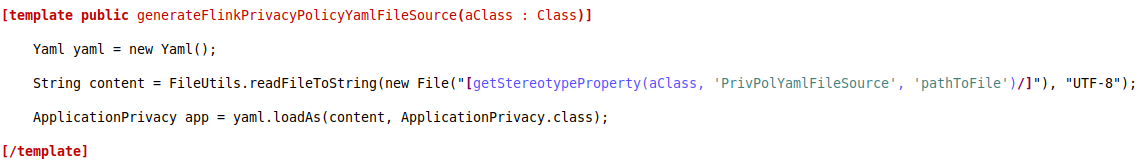
\includegraphics[scale=0.3]{./chapter4/codeStructure/GenerateFlinkPrivacyPolicyYamlFileSource.png}}
\caption{GenerateFlinkPrivacyPolicyYamlFileSource Acceleo Template}
\label{fig:GenerateFlinkPrivacyPolicyYamlFileSource Acceleo Template}
\end{figure}

\begin{figure}
\centering
{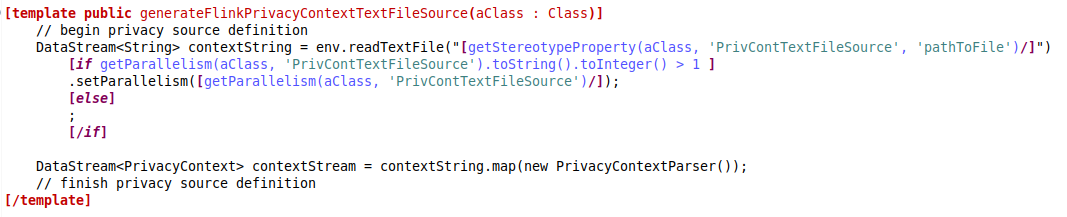
\includegraphics[scale=0.3]{./chapter4/codeStructure/GenerateFlinkPrivacyContextTextFileSource.png}}
\caption{GenerateFlinkPrivacyContextTextFileSource Acceleo Template}
\label{fig:GenerateFlinkPrivacyContextTextFileSource Acceleo Template}
\end{figure}

\subsubsection{Streams Declaration}

After generating and parsing the SCVs and the privacy policy YAML file in the Privacy Policy Initialization part, StreamGen is going to declare all those streams that are introduced to a transformation and that the PrivacyProtectingStream stereotype is not applied on them. In order to do this, another condition must be taken into account as any stream of a DIA which is not privacy policy aware satisfies the condition and, in that case, the streams must not be declared.

Thus, any time that a transformation is generated, after generating the piece of code corresponding to the transformation, two conditions are taken into account. The first condition checks that the input stream of the transformation is not a PrivacyProtectingStream. The second condition checks that exists at least one PrivacyProtectingStream stereotype in the application model. If both conditions are satisfied then the stream is set into the privacy policy YAML file.






